\scanpage{66}
\mspage{32}
$3^\circ)$ \uline{Case \unsure{of|of the}} $\widehat M^!_{0,5}$, or $\widehat M_{0,I}$
\diagram{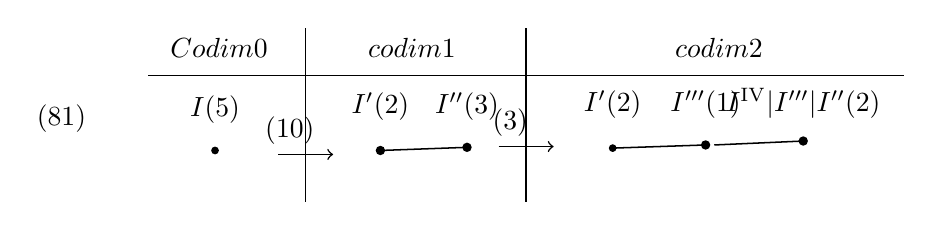
\begin{tikzpicture}[x=1cm,y=1cm,line width=.55pt]
\node at (-1.1,.4) {$(81)$};
\draw (0,.95)--(9.6,.95);
\draw (2,1.55)--(2,-.65);
\draw (4.8,1.55)--(4.8,-.65);
\node at (.9,1.3) {$\text{Codim }0$};
\node at (3.35,1.3) {$\text{codim }1$};
\node at (7.25,1.3) {$\text{codim }2$};
\fill (.85,0) circle (1.4pt);
\node[above] at (.85,.22) {$I(5)$};
\draw[->] (1.65,-.05)--(2.35,-.05);
\node[above] at (1.8,-.05) {$(10)$};
\draw (2.95,0)--(4.05,.04);
\fill (2.95,0) circle (1.7pt);
\fill (4.05,.04) circle (1.7pt);
\node[above] at (2.95,.26) {$I'(2)$};
\node[above] at (4.05,.26) {$I''(3)$};
\draw[->] (4.45,.05)--(5.15,.05);
\node[above] at (4.6,.05) {$(3)$};
\draw (5.9,.03)--(7.08,.07);
\draw (7.19,.07)--(8.32,.12);
\fill (5.9,.03) circle (1.4pt);
\fill (7.08,.07) circle (1.7pt);
\fill (8.32,.12) circle (1.7pt);
\node[above] at (5.9,.28) {$I'(2)$};
\node[above] at (7.08,.28) {$I'''(1)$};
\node[above] at (8.32,.28) {$\unsure{I^{\mathrm{IV}}|I'''|I''}(2)$};
\end{tikzpicture}}
In \unsure{of|the} $\widehat M^!_{0,5}$ there are ten ``divisors at infinity'', each of which is an $\widehat M^!_{0,4}$ \deleted{\unsure{$\simeq\mathbb P$}}, \deleted{\unsure{$\mathbb P^1_{0,3}\mathfrak S_3$}} \inserted{(more precisely, an $\widehat M_{0,I''(3)\amalg(*)}\simeq(\mathbb P^1_{I''})_{\mathbb Z}$)} (having as we had seen, and \unsure{had|would have}) three points at infinity --- the points at infinity number $\frac{30}{2}=15$ in total, corresponding to the partitions of $I(5)$ of type $(2,2,1)$, whereas the divisors at infinity correspond to the subsets \inserted{$I'$} of $I$ of cardinality $2$. Two such divisors, corresponding to subsets $I',I''\in\mathfrak P_2(I)$, meet if and only if \deleted{they} we have $I'\cap I''=\phi$, i.e. \unsure{if and only if|\deleted{if and only if}} $I',I''$ and $I\smallsetminus(I'\cup I'')$ form precisely a partition of $I$ of type $(2,2,1)$.
\margin{$\mathbb P^1_{I''}\overset{\mathrm{def}}{=}\mathbb P^1_{\mathbb Z}\wedge_{\mathfrak S_3}\operatorname{Isom}(\{0,1,\infty\},I'')$}

According to the combinatorial study of the icosahedron, \unsure{choosing|let us choose} an orientation of $I$ --- which determines an oriented icosahedron, or else a skew icosahedron) the $10$ divisors at infinity \deleted{\unsure{in order}} of $\widehat M_{0,I}$, i.e. the \inserted{$10$} \unsure{elements|elements} of $\mathfrak P_2(I)$, \inserted{or (by} \deleted{\unsure{correspon-}}
\margin{65}
